\documentclass[a4paper,twocolumn,10pt]{article}
% Language setting
% Replace `english' with e.g. `spanish' to change the document language
\usepackage[utf8]{inputenc}
\usepackage[spanish]{babel}

% Useful packages
\usepackage{amsmath}
\usepackage{graphicx}
\usepackage{url}

% Title and author info
\title{Taller 2 }
\author{Jose David Ramirez Beltran - 506222723\\Camila Andrea Galindo Ruiz - 506222700\\Miguel Daniel Ruiz Silva - 506222719}

\begin{document}
\maketitle

\section{Introducción}
El término temporal spatial o espacio temporal, en programación se refiere a dos dimensiones cruciales para comprender y optimizar el rendimiento de un programa o algoritmo. Estas especificaciones son esenciales para garantizar que una aplicación funcione eficazmente y se ajuste a las limitaciones de tiempo y espacio disponibles. Mientras que la dimensión espacial se refiere a la cantidad de memoria o espacio de almacenamiento necesario para ejecutar el programa, la dimensión temporal tiene que ver con la velocidad y la eficacia del programa. Estos dos factores deben tenerse en cuenta al desarrollar software en diversos sectores, desde aplicaciones móviles a sistemas, para lograr un equilibrio óptimo entre velocidad de ejecución y eficiencia de recursos.

La gestión de estas dimensiones temporales y espaciales implica tomar decisiones informadas sobre cómo gestionar los recursos informáticos, cómo almacenar y acceder a los datos y cómo diseñar algoritmos para lograr un rendimiento óptimo.


\section{Código en Java}

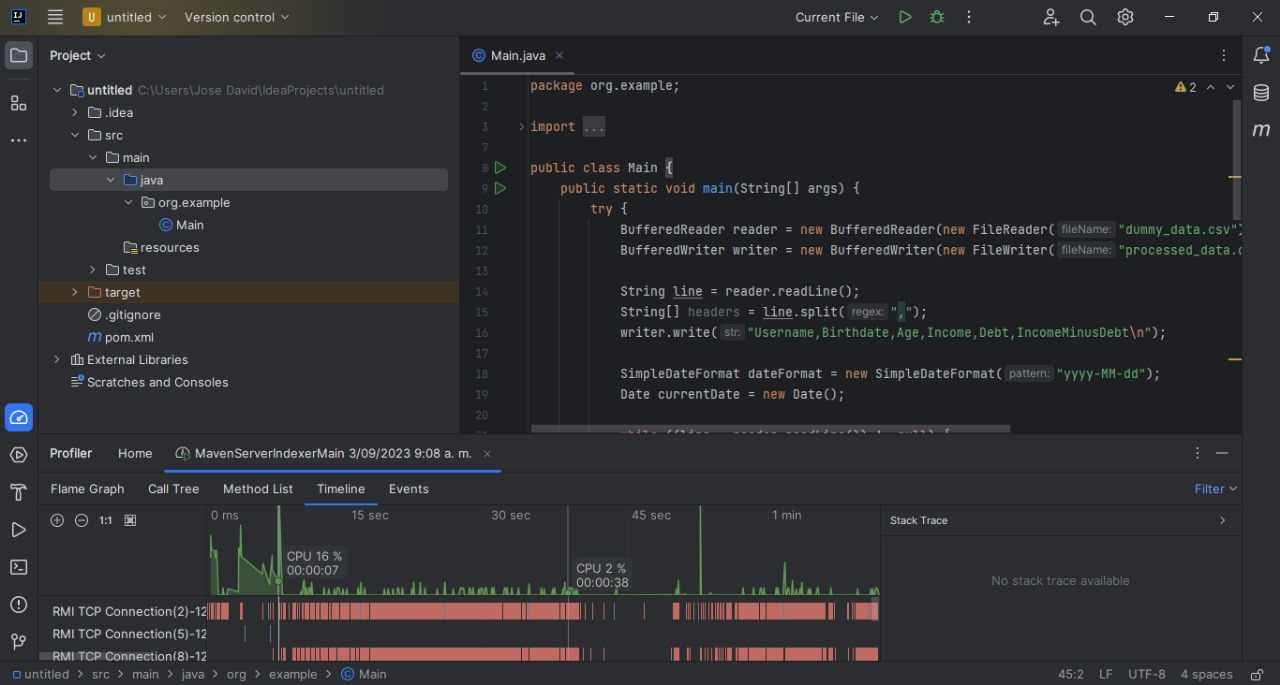
\includegraphics[width=0.85\linewidth]{HP AMD E1-1200 APU/java.jpg}

\begin{itemize}

\item \textbf{Resultado 1}
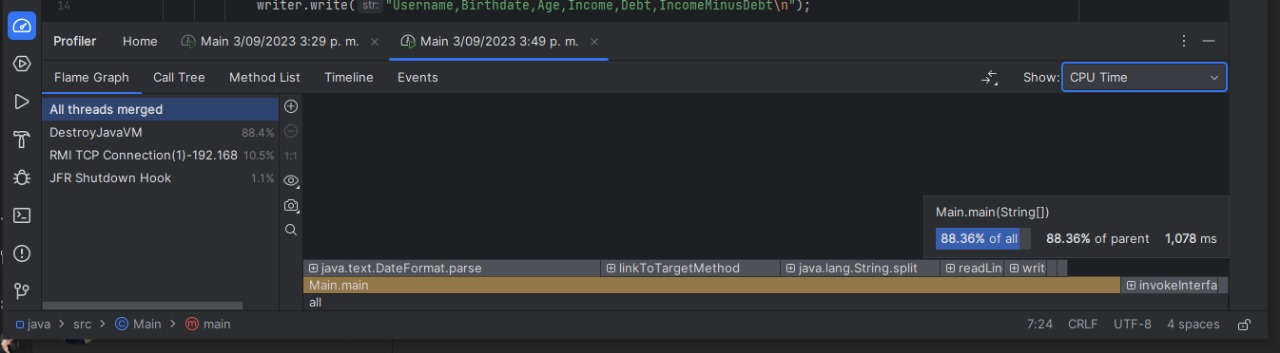
\includegraphics[width=0.85\linewidth]{HP AMD E1-1200 APU/temporaljava.jpg}
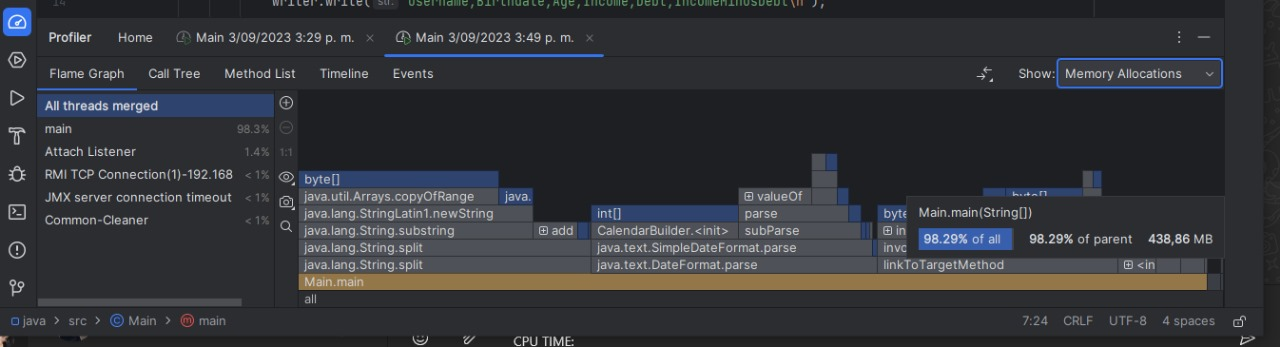
\includegraphics[width=0.85\linewidth]{HP AMD E1-1200 APU/espacialjava.jpg}


\item \textbf{Resultado 2}
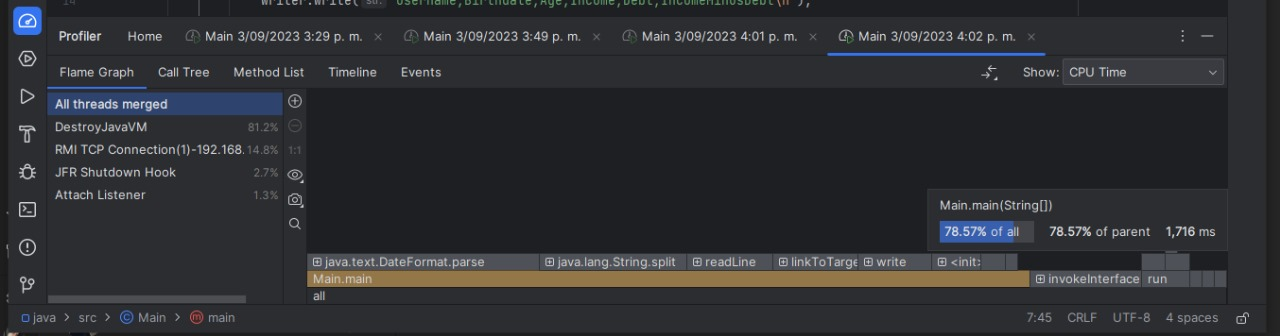
\includegraphics[width=0.85\linewidth]{HP AMD E1-1200 APU/resultado.2.jpg}
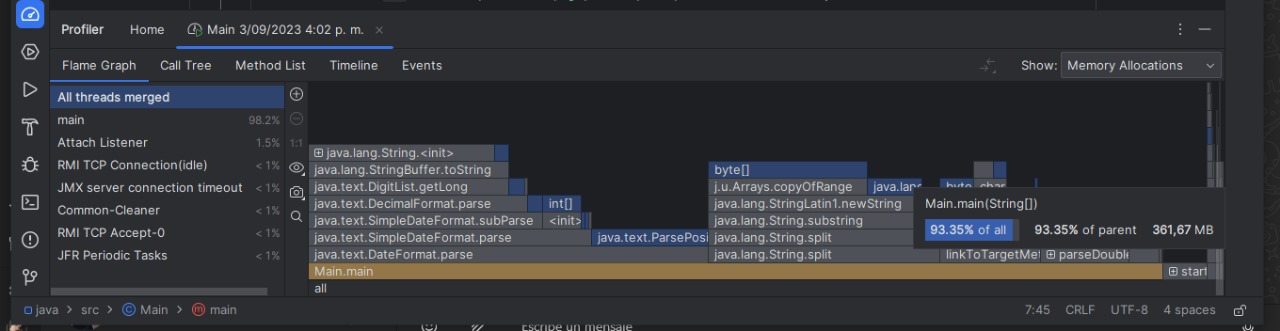
\includegraphics[width=0.85\linewidth]{HP AMD E1-1200 APU/resultado2.jpg}


\item \textbf{Resultado 3}
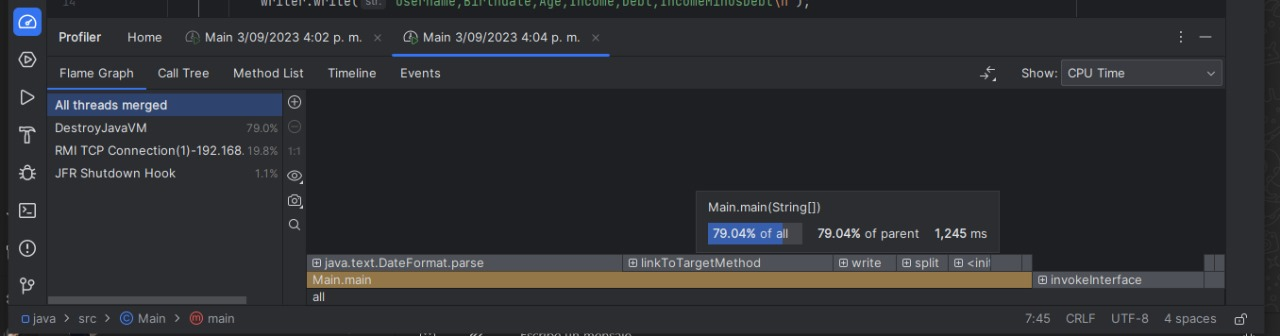
\includegraphics[width=0.85\linewidth]{HP AMD E1-1200 APU/resultado.3.jpg}
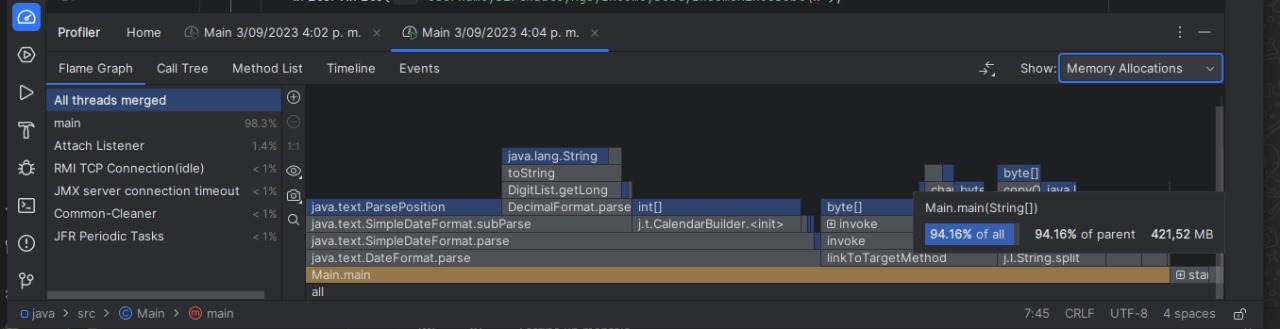
\includegraphics[width=0.85\linewidth]{HP AMD E1-1200 APU/r3.jpg}


\item Complejidad Temporal


\item La lectura del archivo de entrada línea por línea tiene una complejidad temporal lineal (\(O(n)\)), donde \(n\) es el número de líneas en el archivo \texttt{dummy\_data.csv}.
    \item La división de cada línea en valores utilizando \texttt{split(",")} también tiene una complejidad lineal en relación con el número de caracteres en la línea, por lo que se puede considerar como \(O(m)\), donde \(m\) es la longitud de la línea más larga.
    \item La conversión de fechas y números tiene una complejidad constante para cada línea, por lo que no contribuye significativamente al análisis de complejidad.
    \item El cálculo de la edad y la resta de ingresos y deuda también tienen una complejidad constante por línea.
    \item Dado que estas operaciones se realizan para cada línea del archivo, podemos decir que la complejidad temporal total depende principalmente del número de líneas en el archivo \texttt{dummy\_data.csv}, es decir, es lineal en relación con la entrada.

\end{itemize}

\begin{itemize}

\item Complejidad Espacial
\item La cantidad de memoria utilizada durante la ejecución está relacionada con la complejidad espacial del programa, en este caso los datos se leen y escriben línea por línea, por lo que el uso de memoria es constante e independiente del tamaño de todo el archivo. Pero, hay que tener en cuenta que las líneas se almacenan en memoria mientras se procesan y se escriben en el archivo de salida.
\item Ya que el programa utiliza un máximo del 16 por ciento de la memoria y se ejecuta en un minuto, podemos deducir que el uso de la memoria es racionalmente eficiente dado el tamaño del archivo de trabajo. En este caso, la complejidad espacial no parece ser un problema significativo.

\end{itemize}


\section{Código Python}

Primera ejecucion

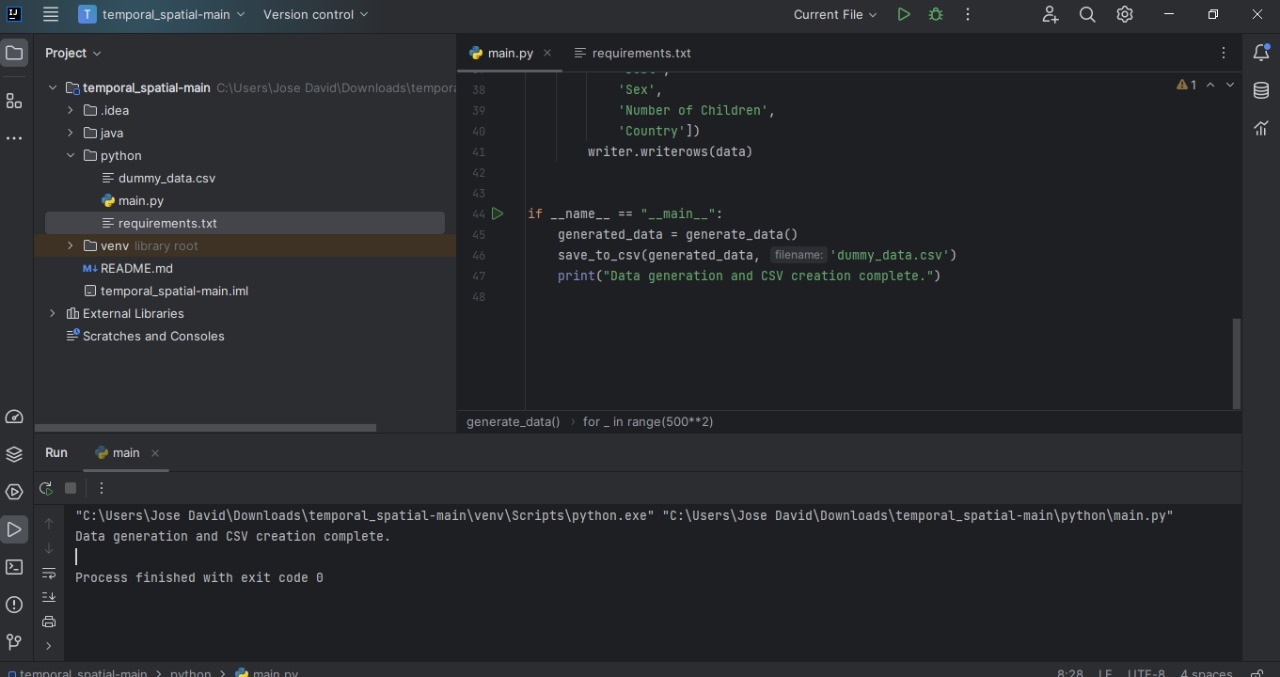
\includegraphics[width=1\linewidth]{HP AMD E1-1200 APU/py1.jpg}

Segunda ejecucion

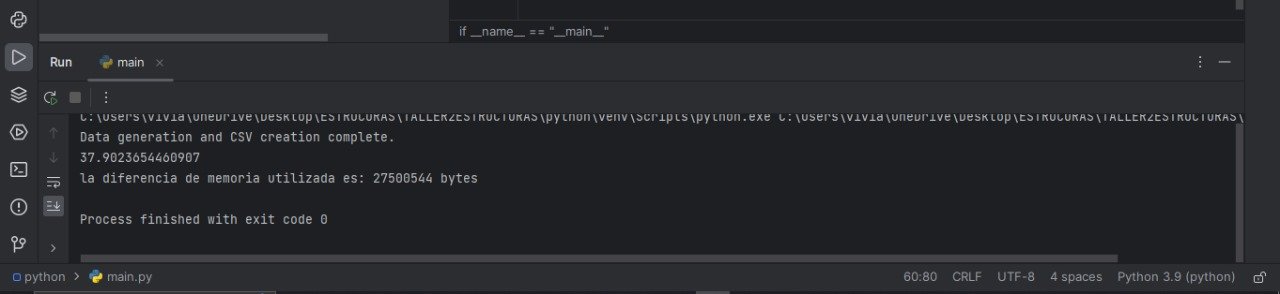
\includegraphics[width=1\linewidth]{HP AMD E1-1200 APU/py2.jpg}

Tercera ejecucion

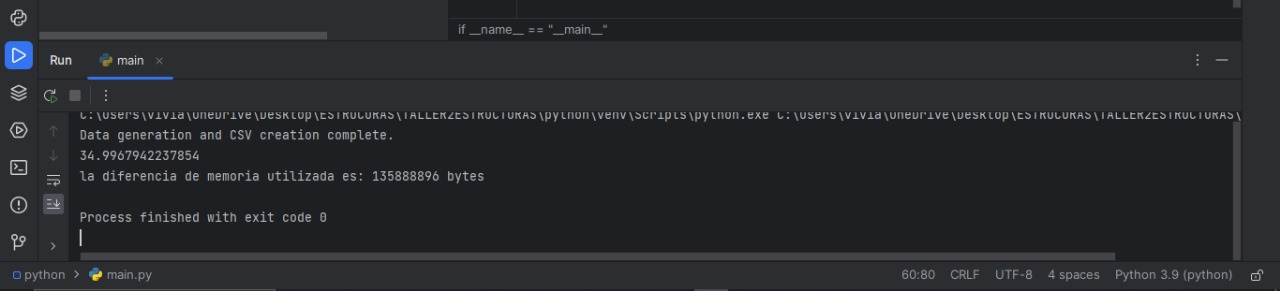
\includegraphics[width=1\linewidth]{HP AMD E1-1200 APU/py3.jpg}

\textbf{Complejidad Temporal:}
\begin{itemize}
    \item El bucle \texttt{for} que genera los datos se ejecuta \(500^2\) veces, lo que significa que genera un total de 250,000 registros de datos ficticios.
    \item Dentro del bucle, se realizan operaciones que son generar un nombre de usuario, fecha de nacimiento, ingreso, deuda, género, número de hijos y país para cada registro, esta generacion es constante en relación con el número de registros que se están generando.
    \item El bucle de escritura a CSV también es lineal en relación con el número de registros (250,000).
\end{itemize}

Dado que todas estas operaciones son lineales en relación con el número de registros, se puede decir que la complejidad temporal es aproximadamente lineal, es decir, \(O(n)\), donde \(n\) es el número de registros generados.

\textbf{Complejidad Espacial:}
\begin{itemize}
    \item El código genera una lista llamada \texttt{data} que almacena todos los registros antes de escribirlos en el archivo CSV. La lista \texttt{data} contiene 250,000 elementos, uno por cada registro generado.
    \item Los datos en la lista \texttt{data} se escriben en un archivo CSV llamado 'dummy\_data.csv' mediante el uso de la función \texttt{save\_to\_csv}.
\end{itemize}

\begin{itemize}
\item Dado que el tamaño de la lista \texttt{data} es proporcional al número de registros generados, la complejidad espacial es \(O(n)\), donde \(n\) es el número de registros. 

\item Por lo tanto, la complejidad temporal es lineal \(O(n)\) y la complejidad espacial también es lineal \(O(n)\), esto significa que tanto el tiempo de ejecución como el uso de memoria aumentan de manera lineal con la cantidad de datos generados. Teniendo en cuenta los datos de la ejecucion parece ser razonablemente eficiente para el tamaño de datos generados.
\end{itemize}



\section{Resultados en diferentes pc}
\maketitle HP ryzen 5500U

\textsc{Python}

\textbf{Ejecución 1\\}
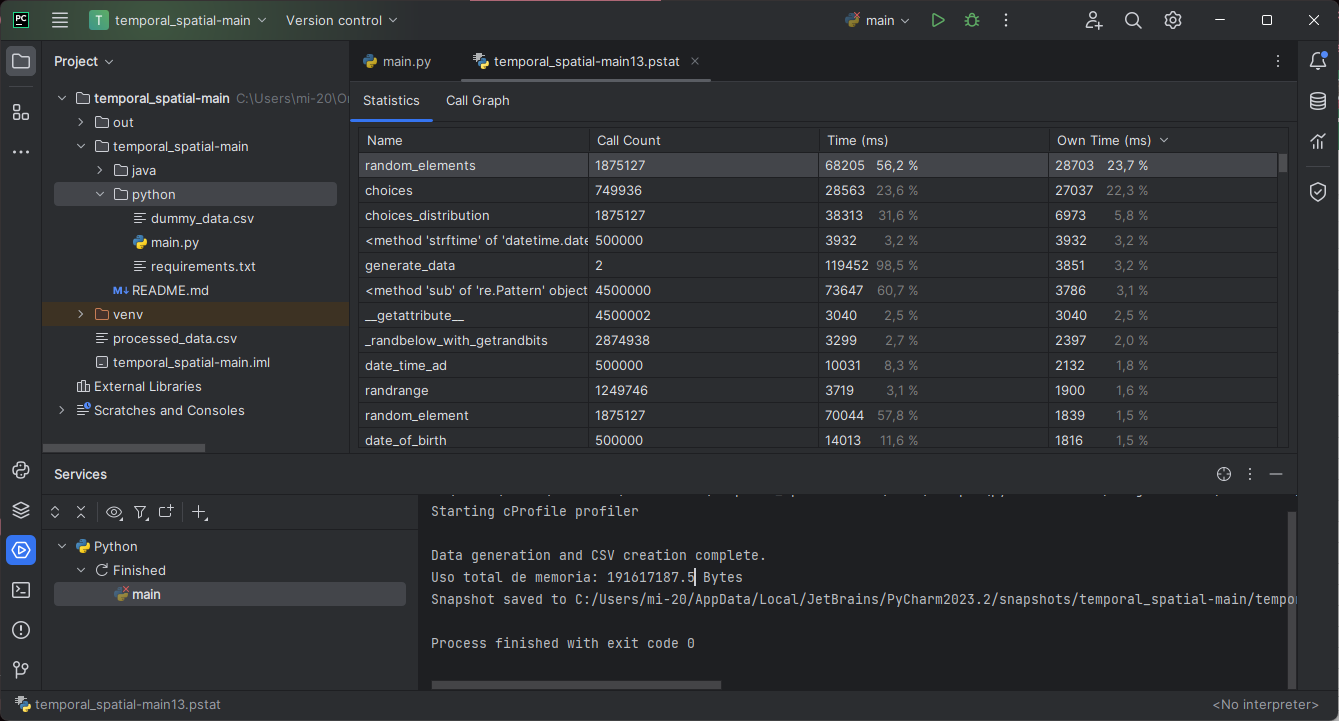
\includegraphics[width=0.9\linewidth]{HP Ryzen 5500U/Prueba python 1.png}

\textbf{Ejecución 2\\}
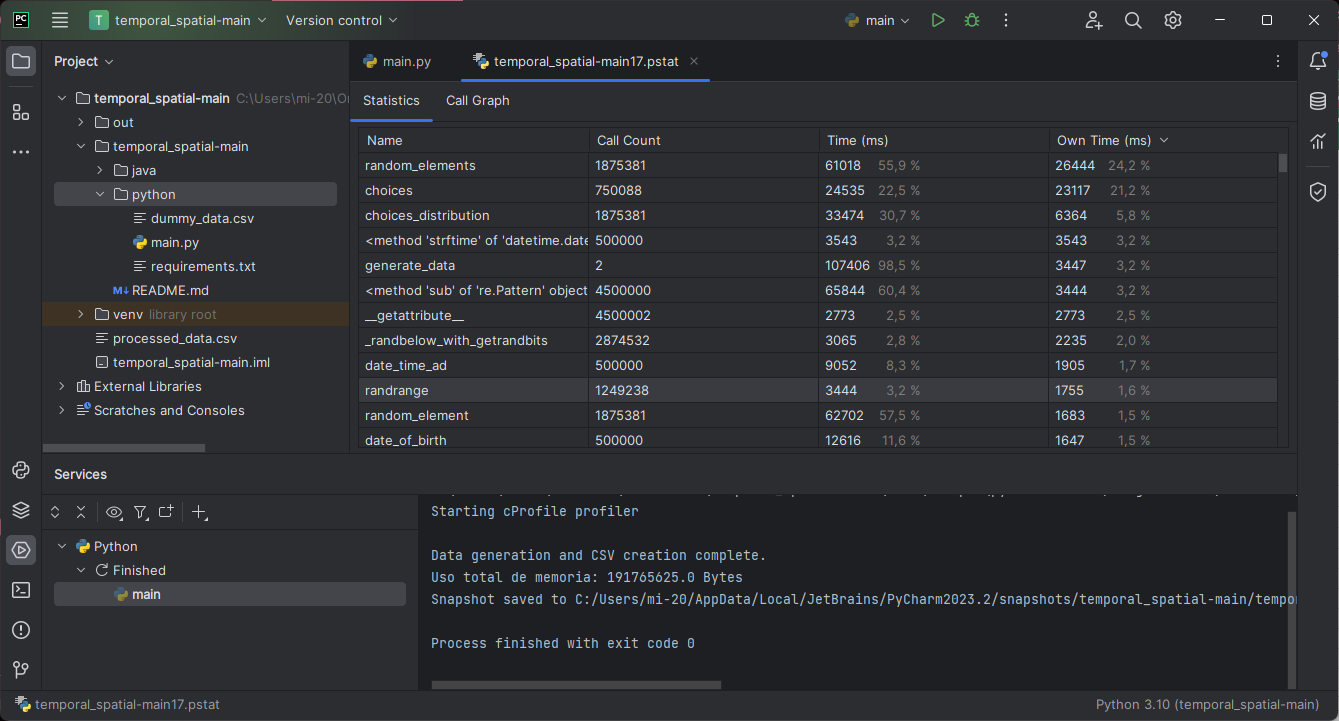
\includegraphics[width=0.9\linewidth]{HP Ryzen 5500U/Prueba python 2.png}

\textbf{Ejecución 3\\}
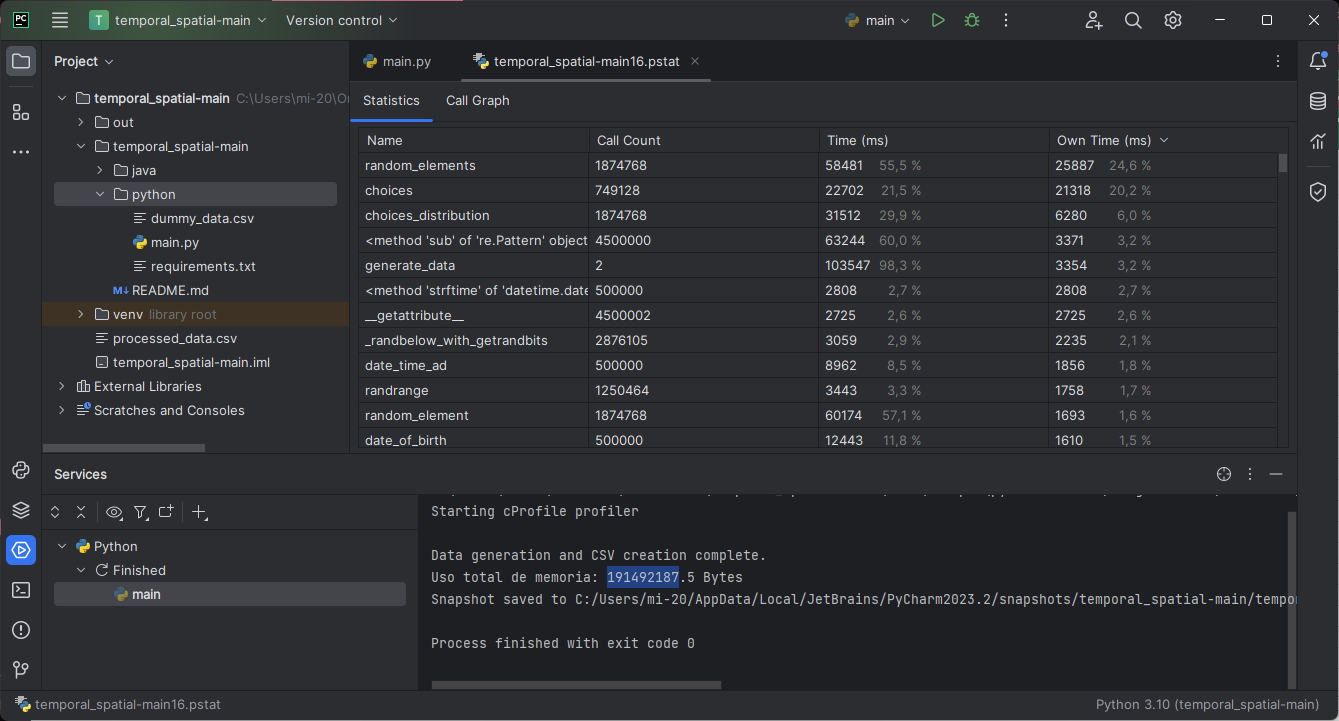
\includegraphics[width=0.9\linewidth]{HP Ryzen 5500U/Prueba python 3.png} 

\textsc{Java}

\textbf{Ejecución 1\\}
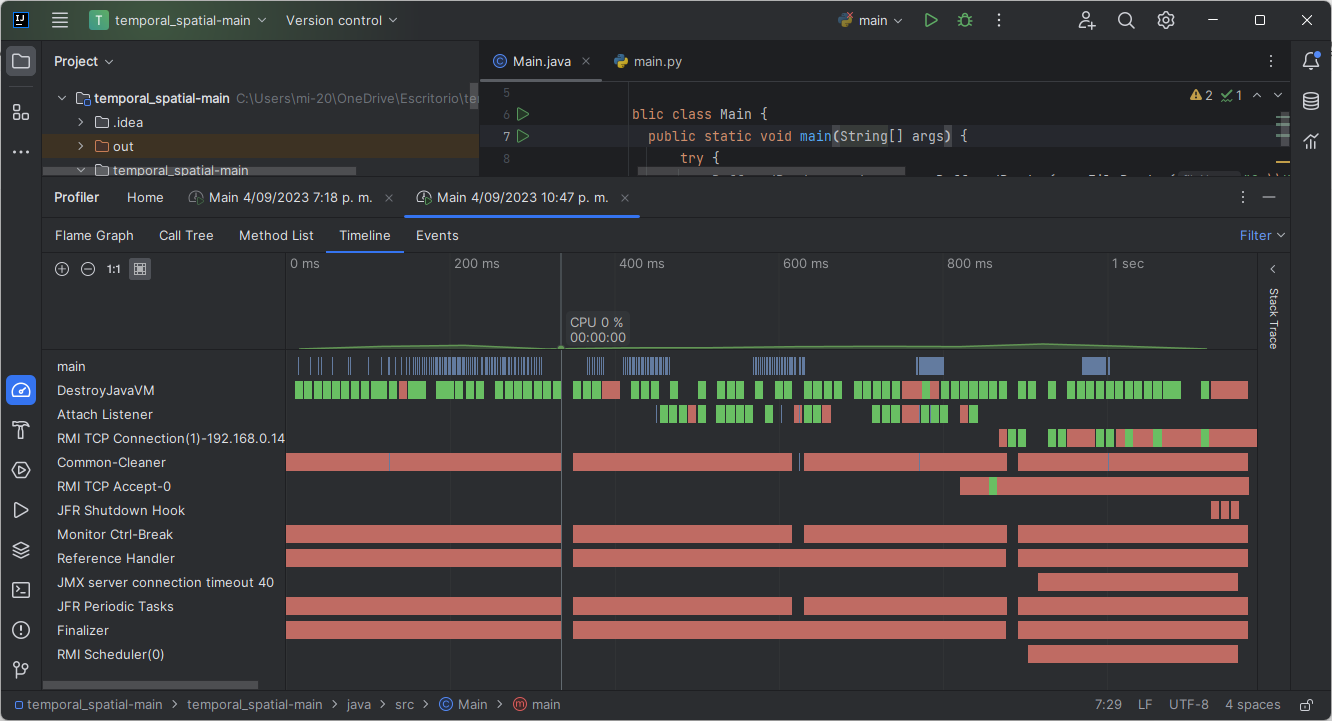
\includegraphics[width=0.9\linewidth]{HP Ryzen 5500U/Timeline 1.png}
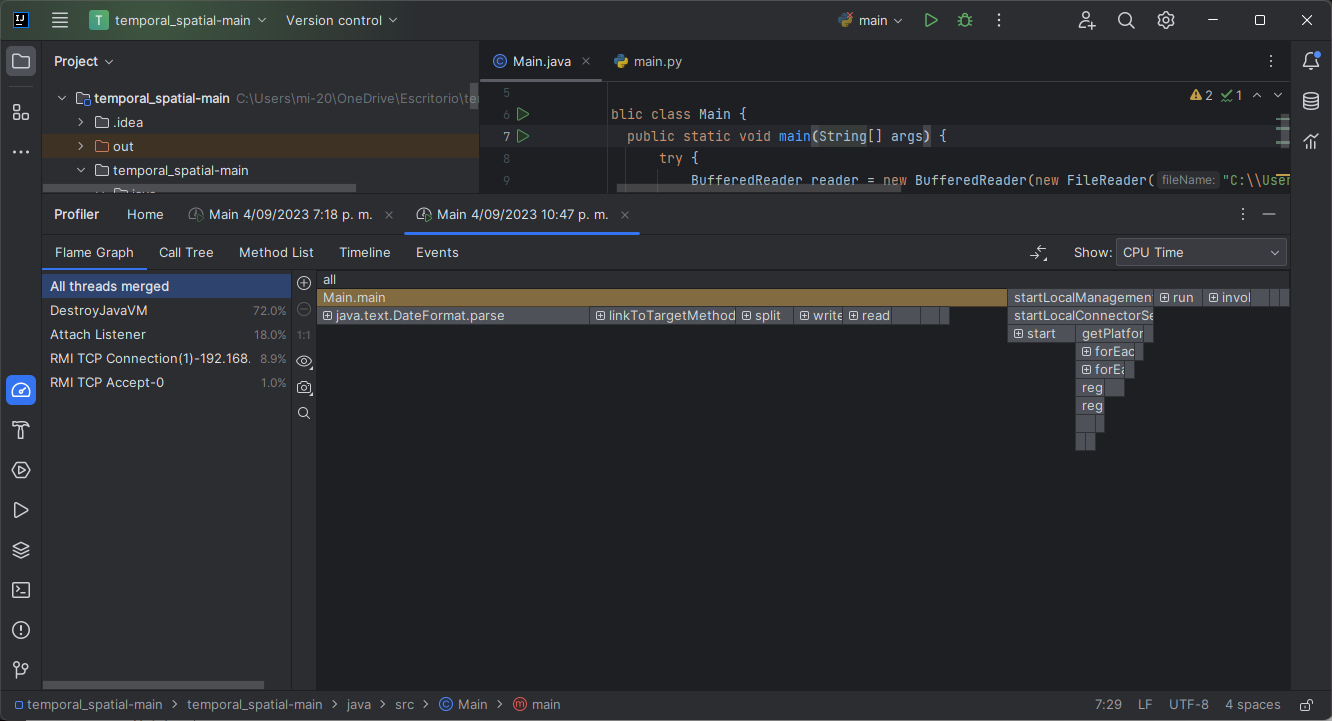
\includegraphics[width=0.9\linewidth]{HP Ryzen 5500U/FlameGraph CPU 1.png}
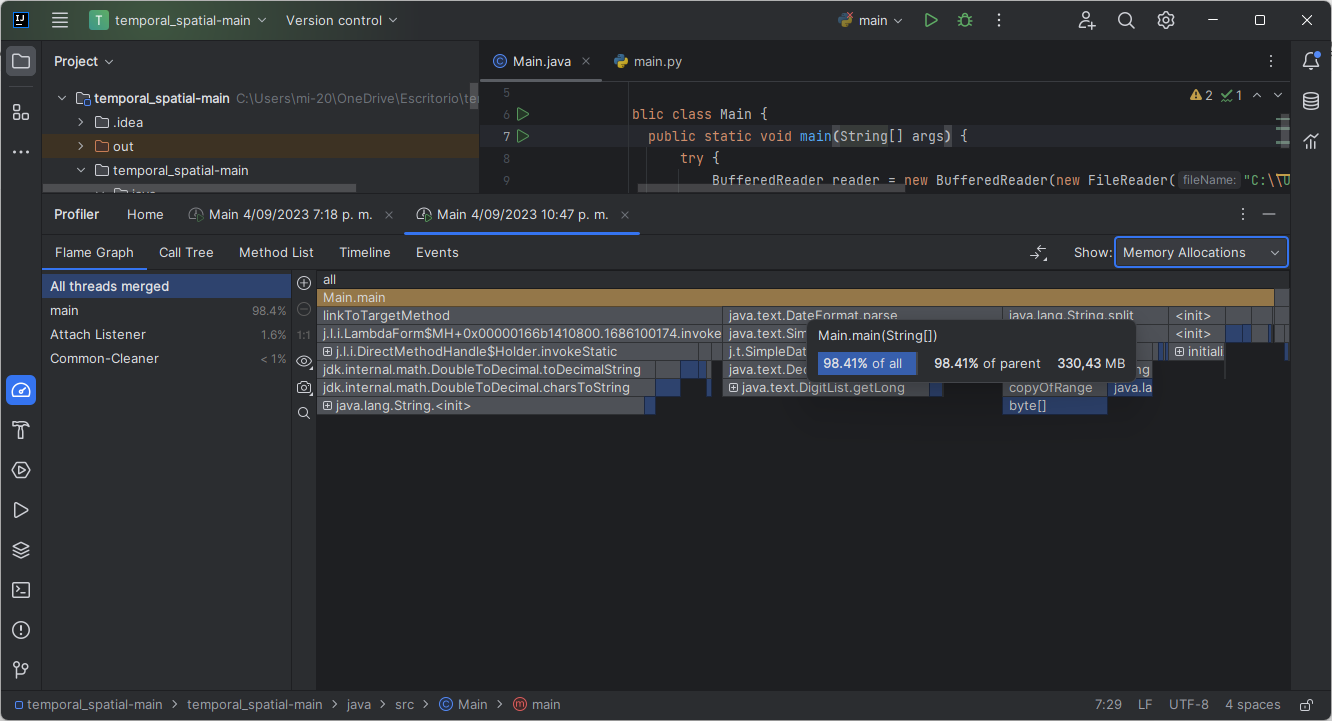
\includegraphics[width=0.9\linewidth]{HP Ryzen 5500U/FlameGraph Memory Allocation 1.png}
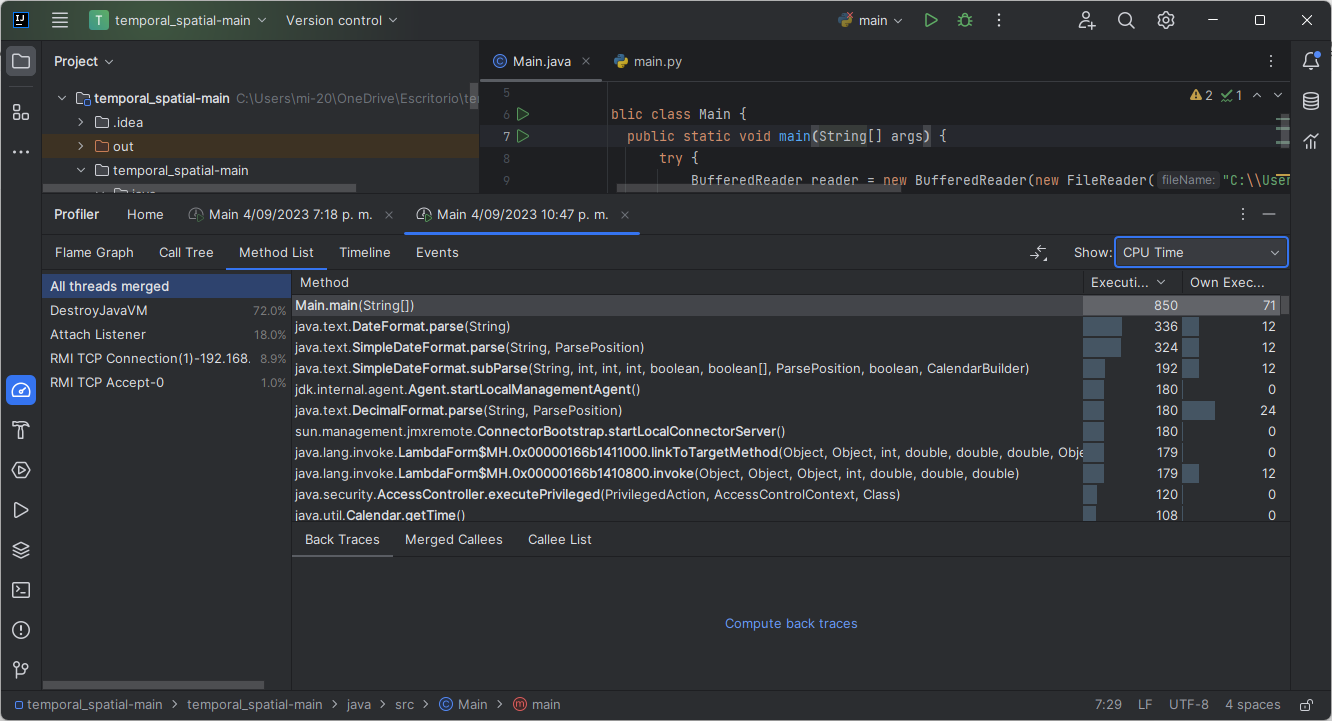
\includegraphics[width=0.9\linewidth]{HP Ryzen 5500U/Method List CPU 1.png}
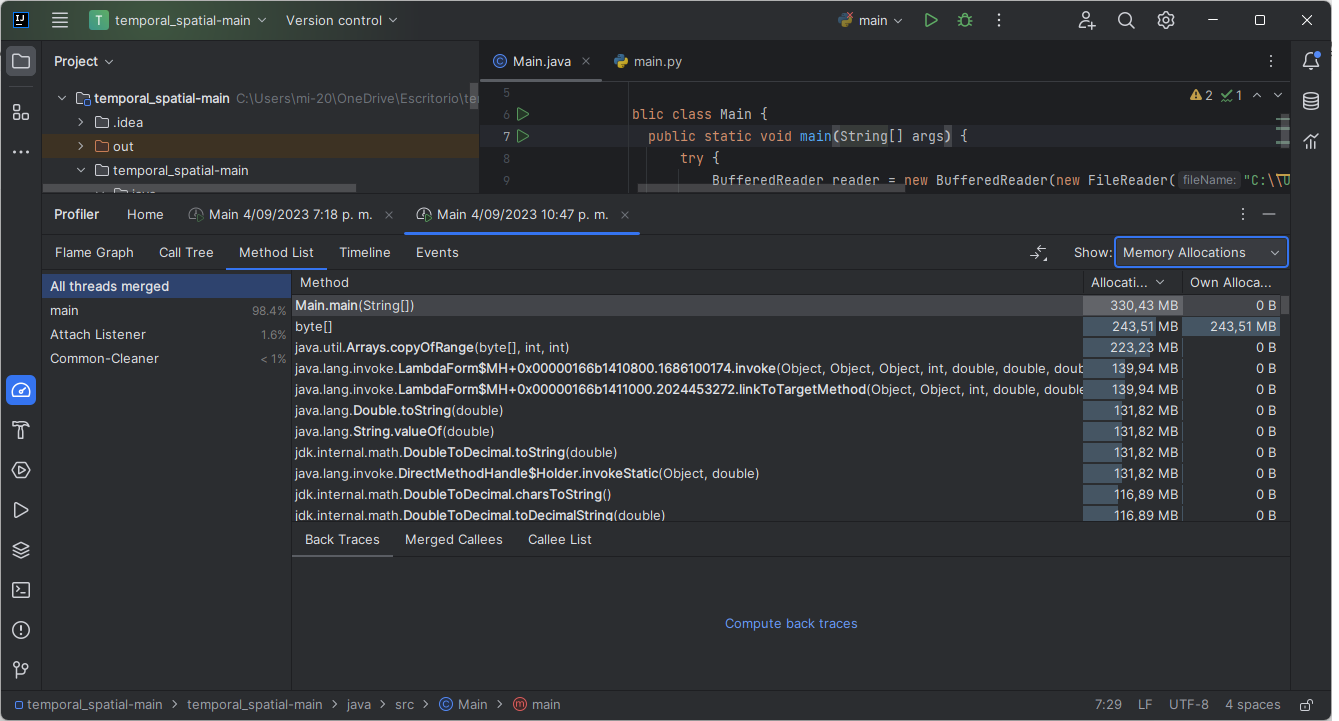
\includegraphics[width=0.9\linewidth]{HP Ryzen 5500U/Method List Memory Allocation 1.png}

\textbf{Ejecución 2\\}
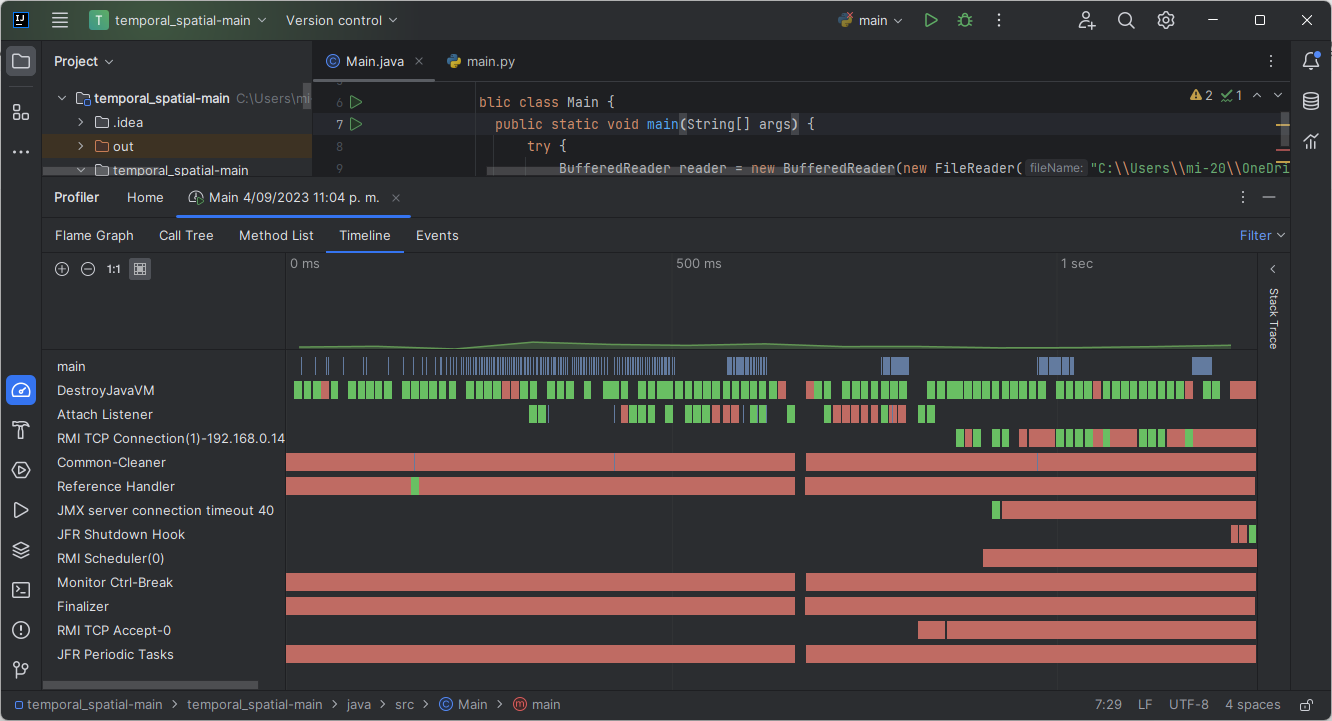
\includegraphics[width=0.9\linewidth]{HP Ryzen 5500U/TimeLine 2.png}
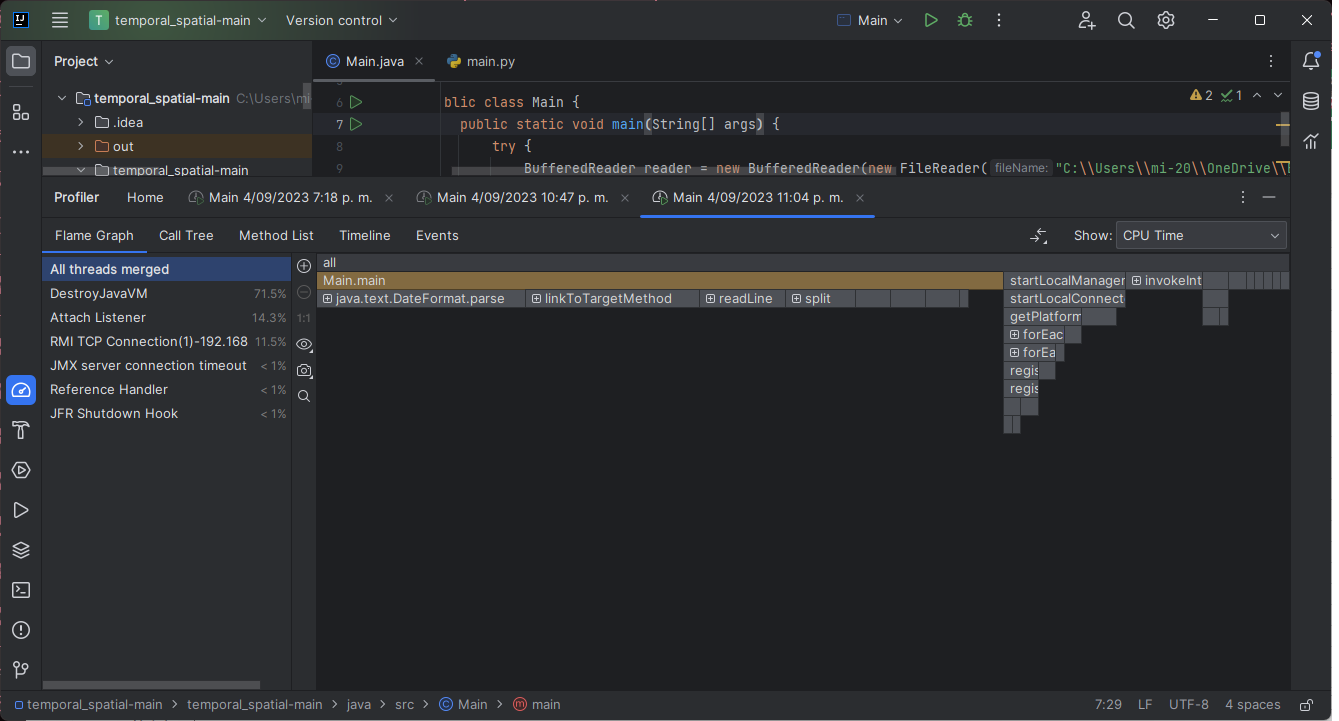
\includegraphics[width=0.9\linewidth]{HP Ryzen 5500U/FlameGraph CPU 2.png}
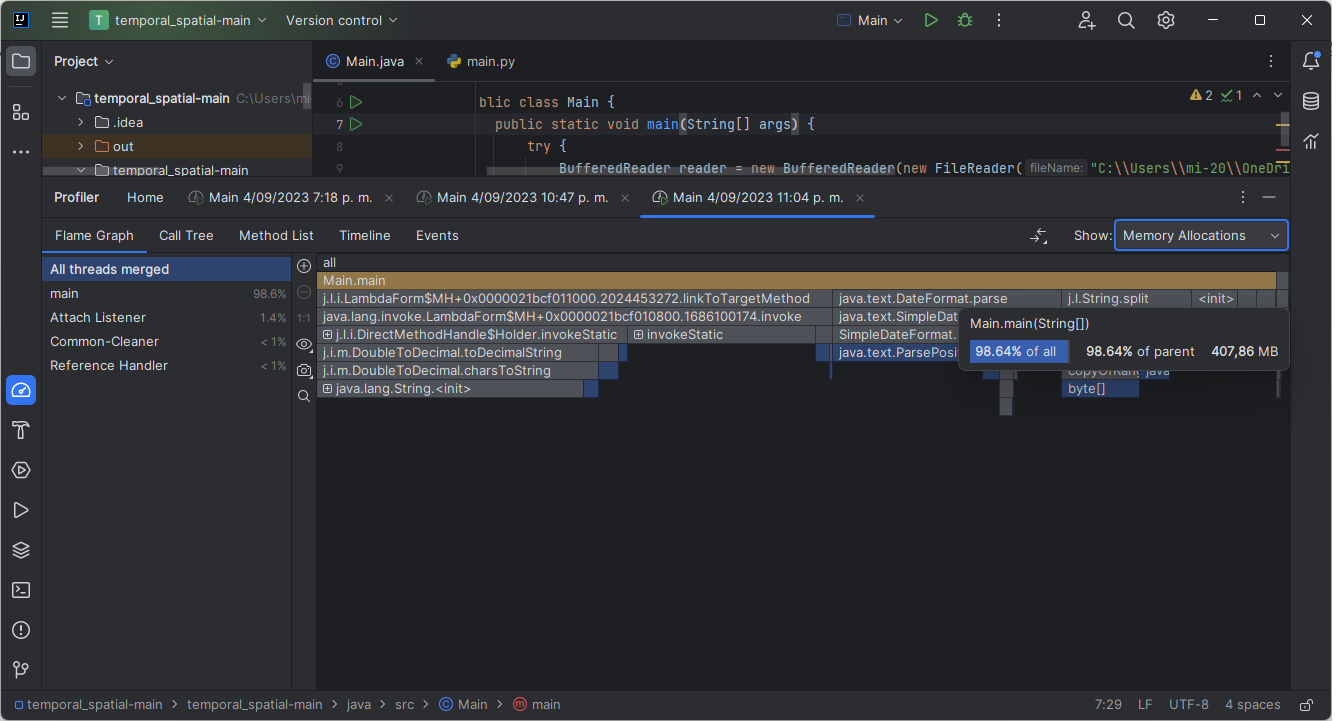
\includegraphics[width=0.9\linewidth]{HP Ryzen 5500U/FlameGraph Memory Allocation 2.png}
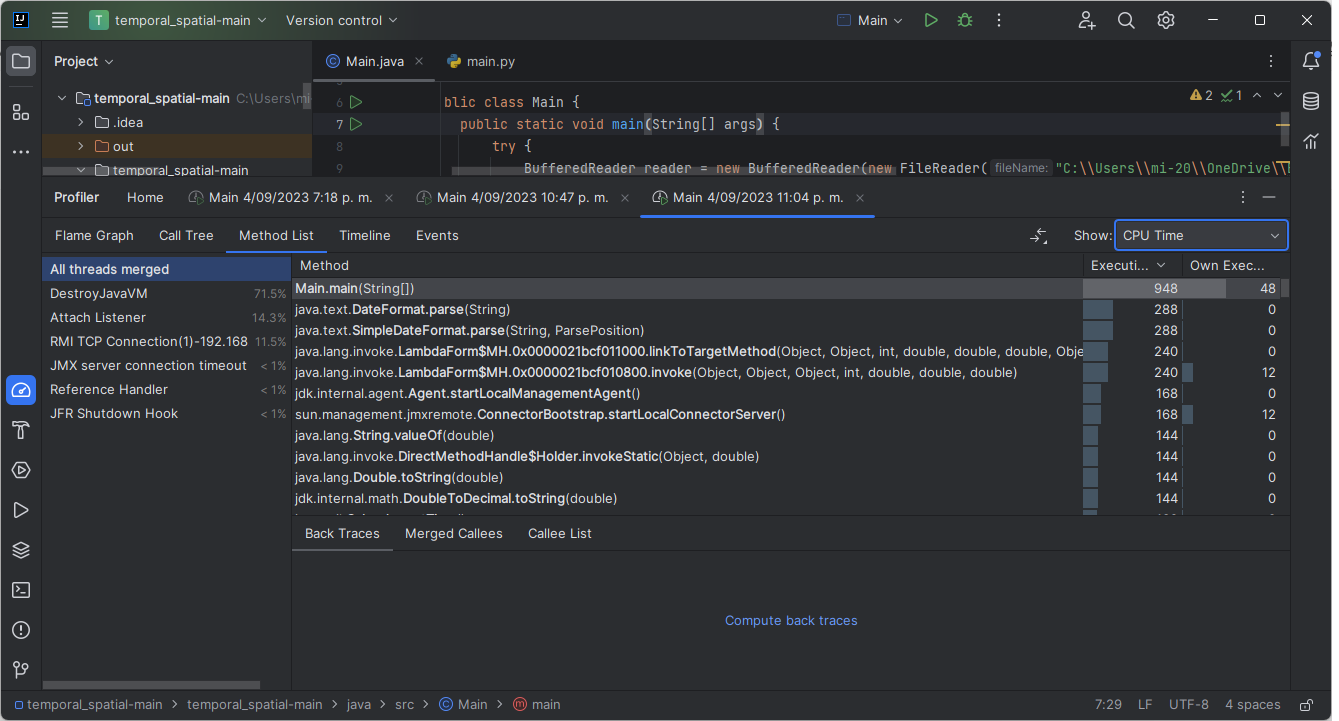
\includegraphics[width=0.9\linewidth]{HP Ryzen 5500U/Method List CPU 2.png}
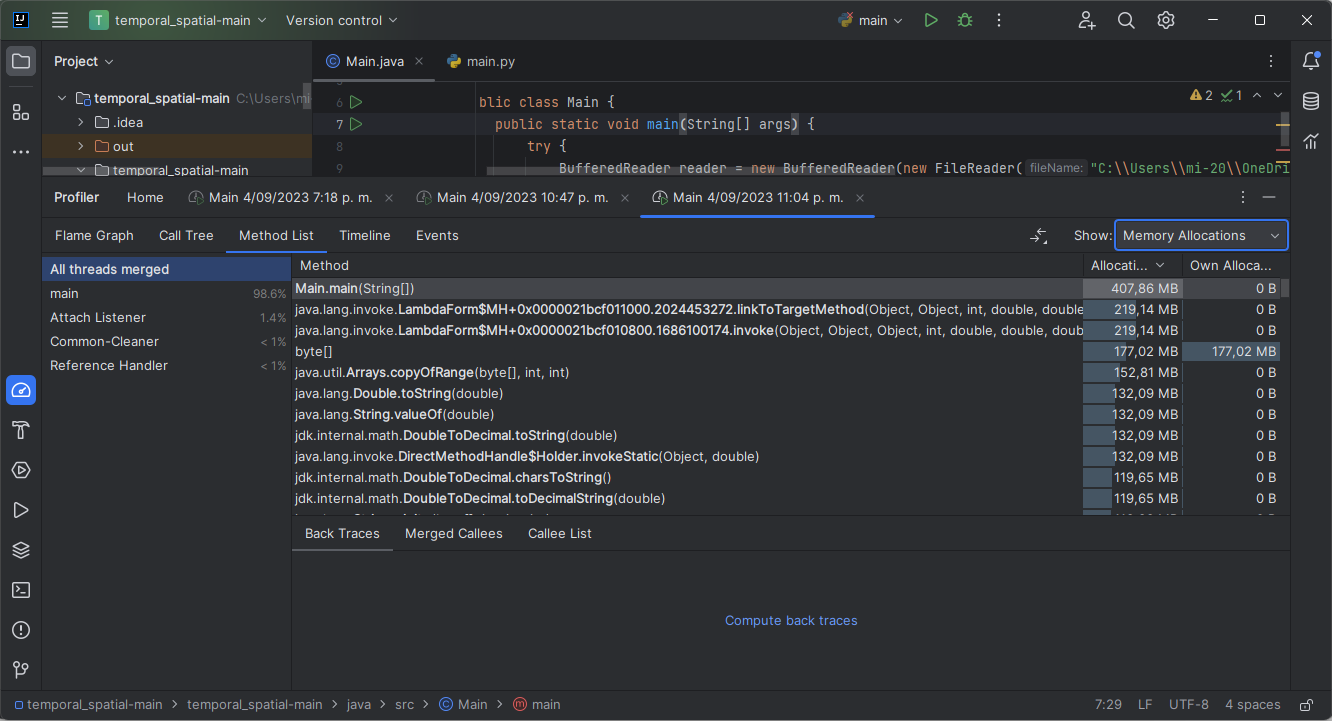
\includegraphics[width=0.9\linewidth]{HP Ryzen 5500U/Method List Memory Allocation 2.png}

\textbf{Ejecución 3\\}
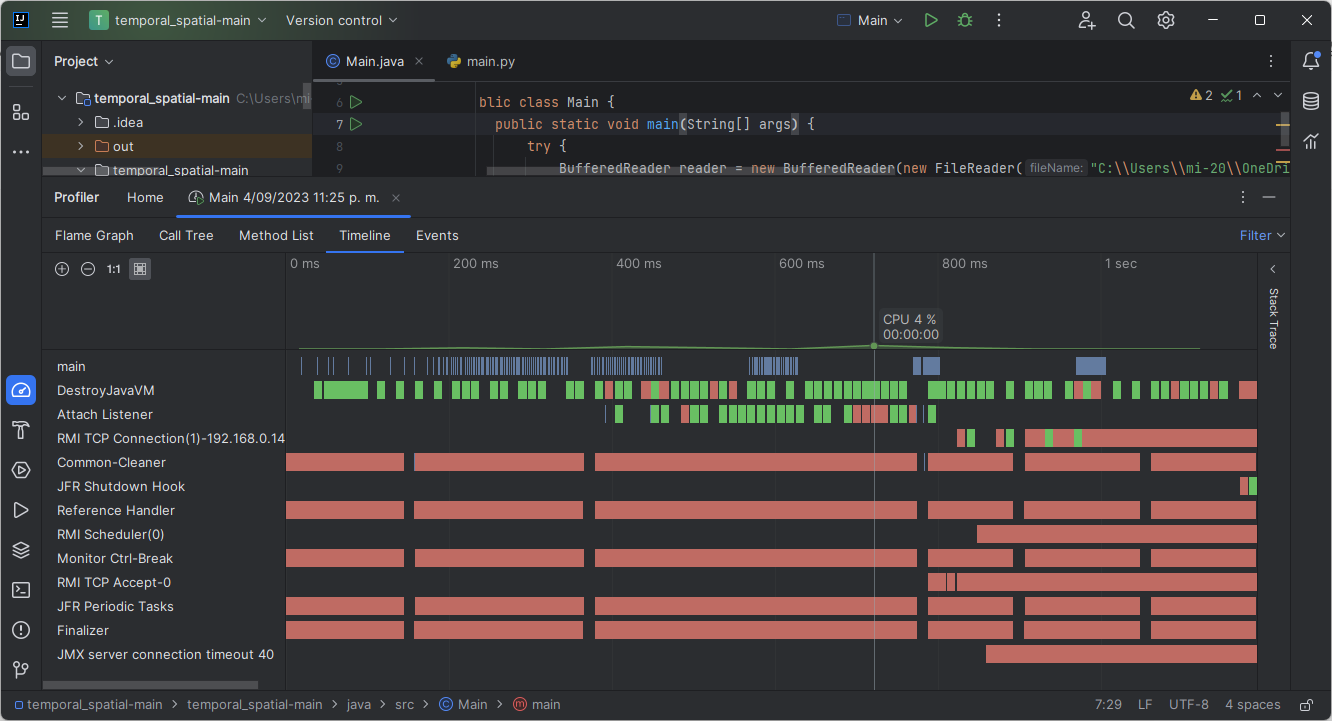
\includegraphics[width=0.9\linewidth]{HP Ryzen 5500U/TimeLine 3.png}
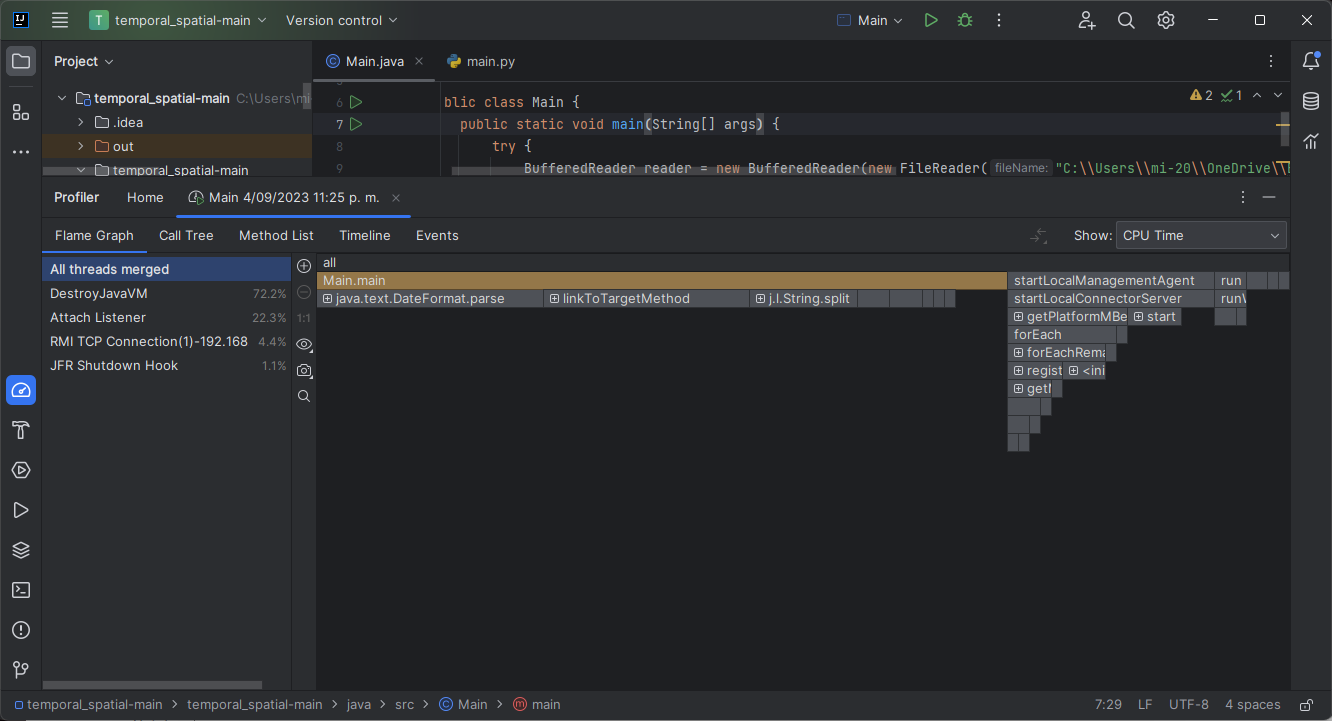
\includegraphics[width=0.9\linewidth]{HP Ryzen 5500U/FlameGraph CPU 3.png}
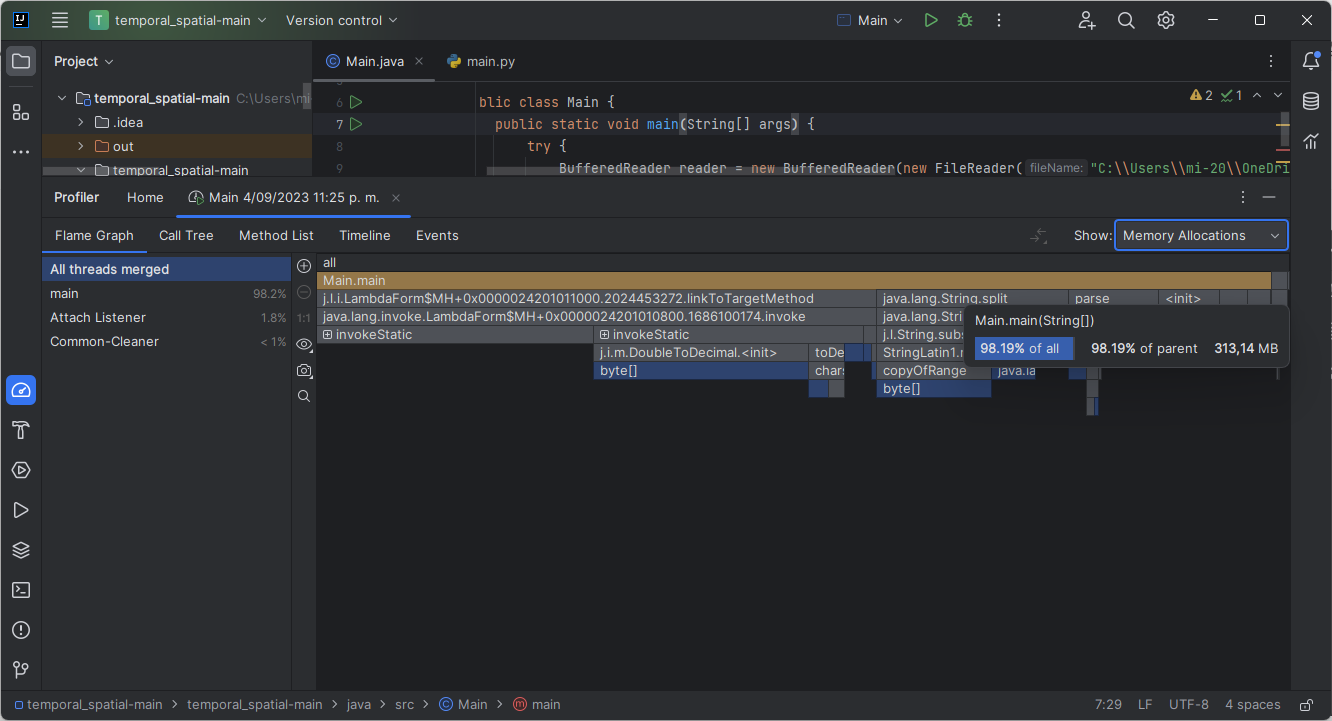
\includegraphics[width=0.9\linewidth]{HP Ryzen 5500U/FlameGraph Memory Allocation 3.png}
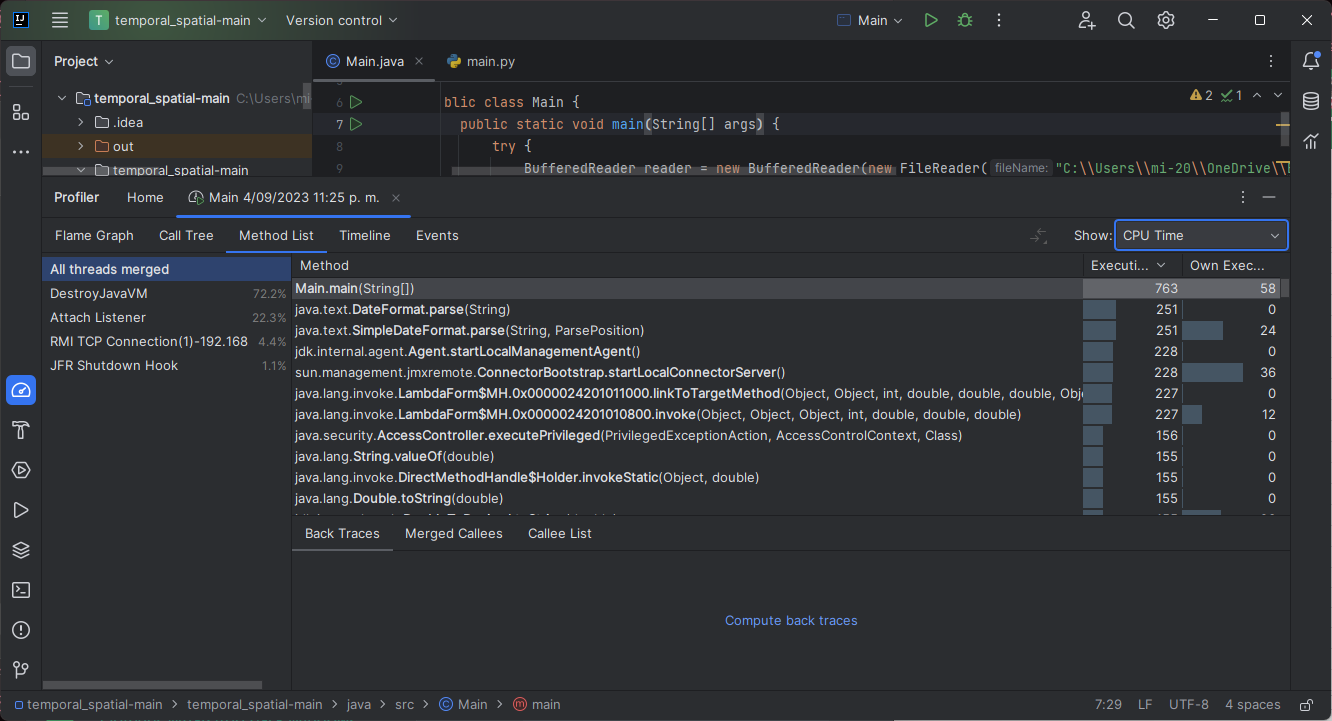
\includegraphics[width=0.9\linewidth]{HP Ryzen 5500U/Method List CPU 3.png}
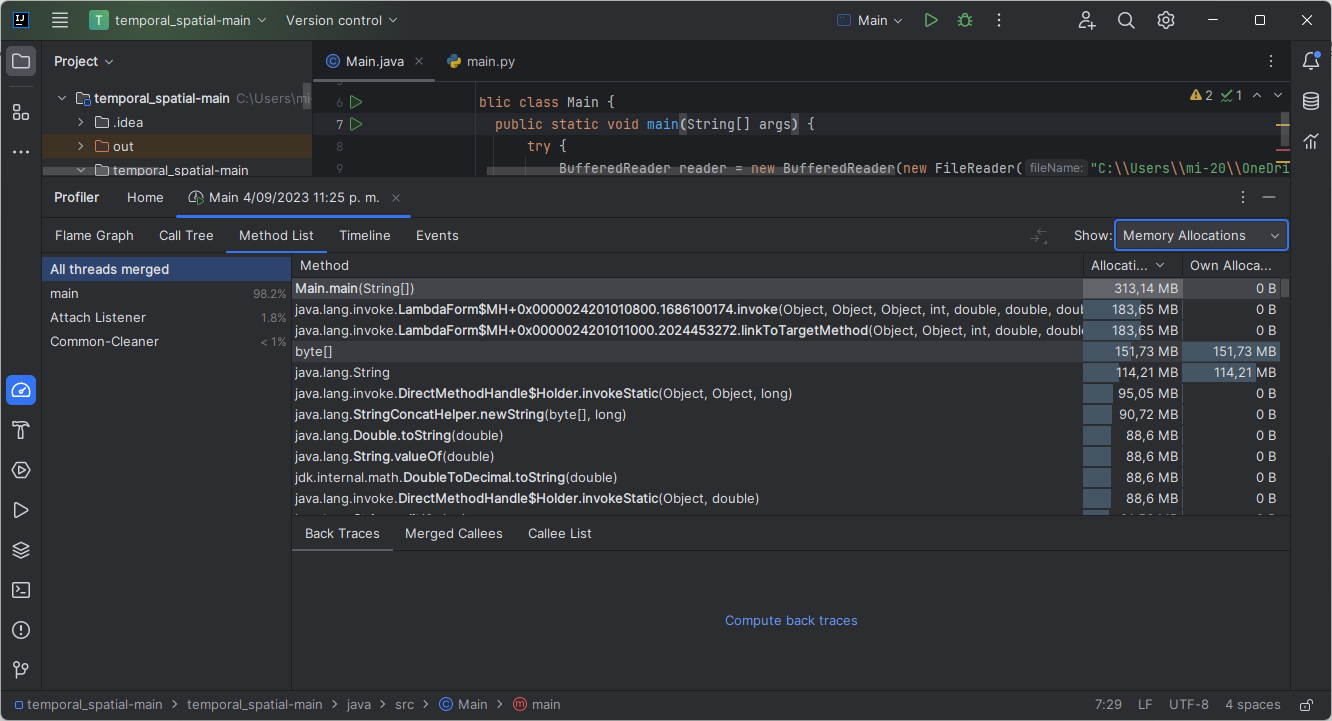
\includegraphics[width=0.9\linewidth]{HP Ryzen 5500U/Method List Memory Allocation 3.png}\\

\maketitle Lenovo AMD 3020e\\

\textsc{Python}

\textbf{Ejecución 1\\}
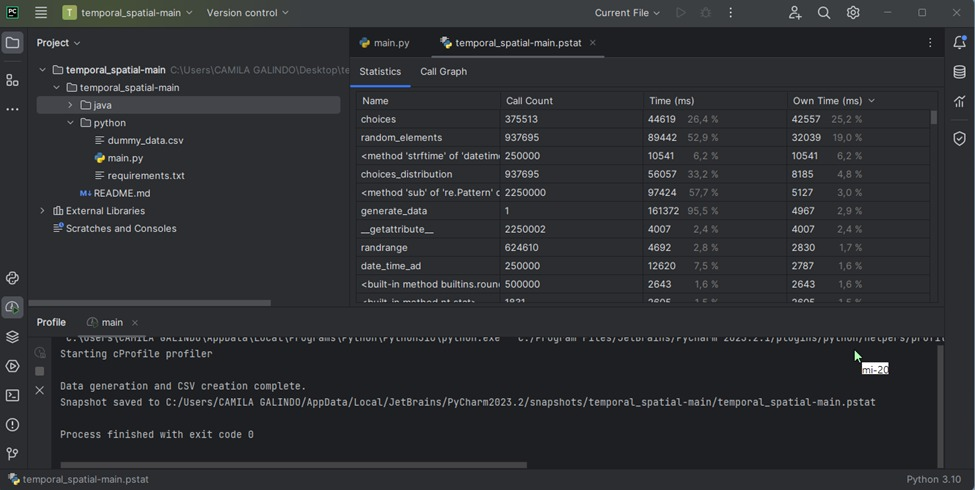
\includegraphics[width=0.9\linewidth]{Lenovo AMD 3020e/Prueba python 1.jpeg}

\textbf{Ejecución 2\\}
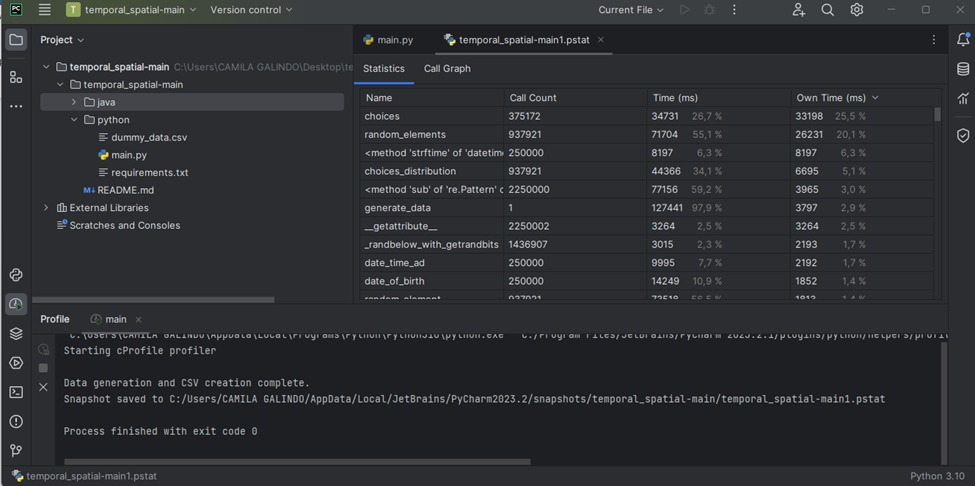
\includegraphics[width=0.9\linewidth]{Lenovo AMD 3020e/Prueba python 2.jpeg}

\textbf{Ejecución 3\\}
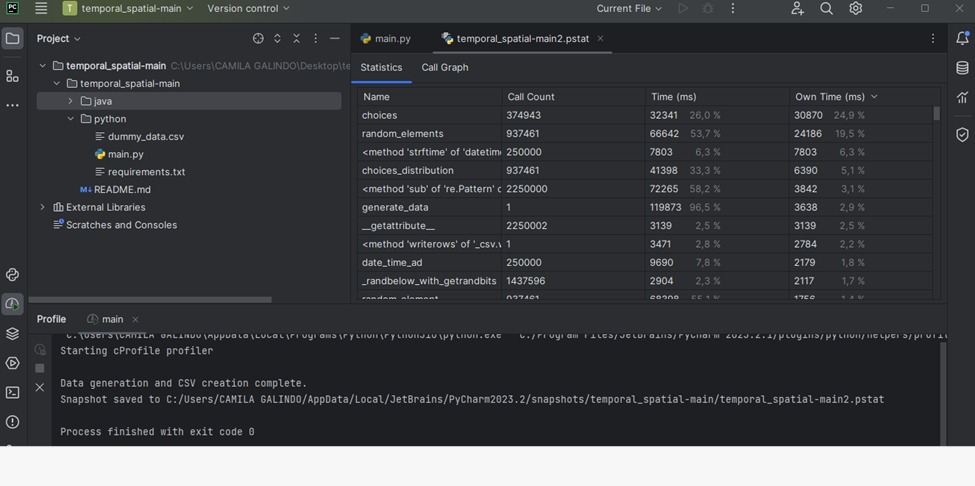
\includegraphics[width=0.9\linewidth]{Lenovo AMD 3020e/Prueba python 3.jpeg}\\

\textsc{Java}

\textbf{Ejecución 1\\}
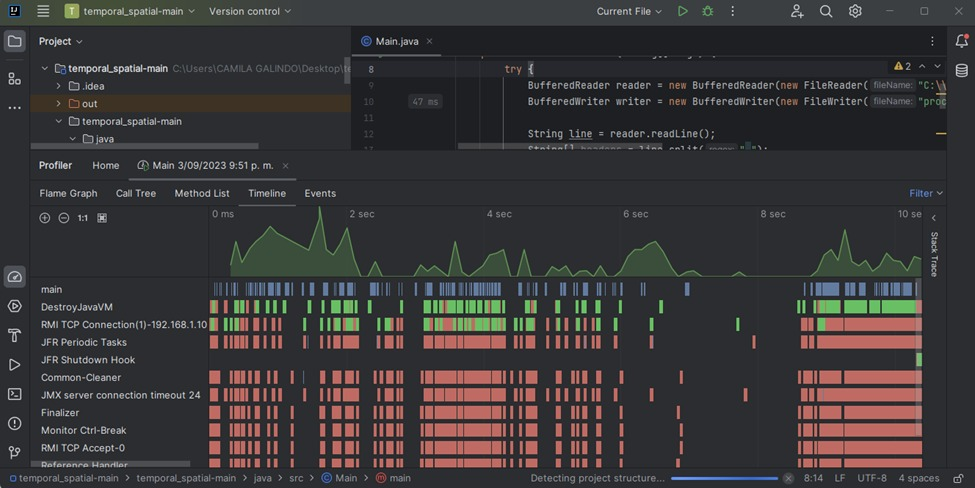
\includegraphics[width=0.9\linewidth]{Lenovo AMD 3020e/TimeLine 1.jpeg}
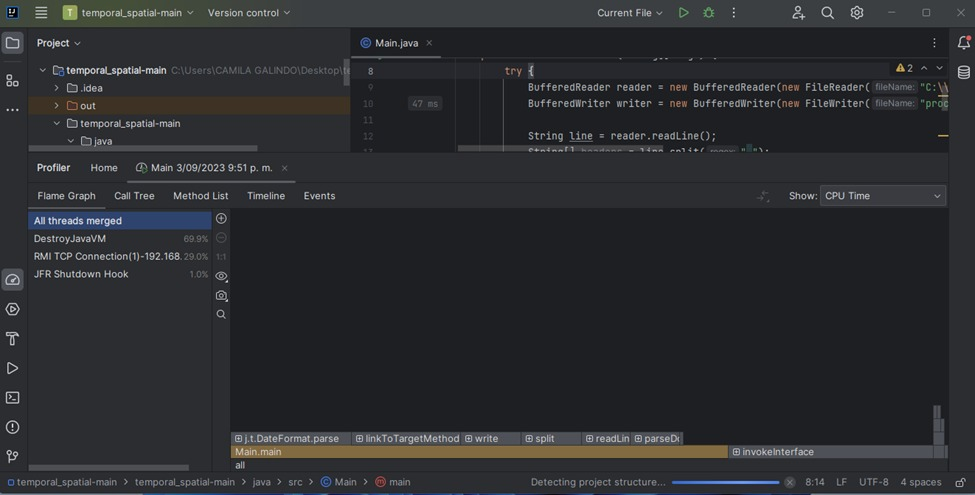
\includegraphics[width=0.9\linewidth]{Lenovo AMD 3020e/FlameGraph CPU Time 1.jpeg}
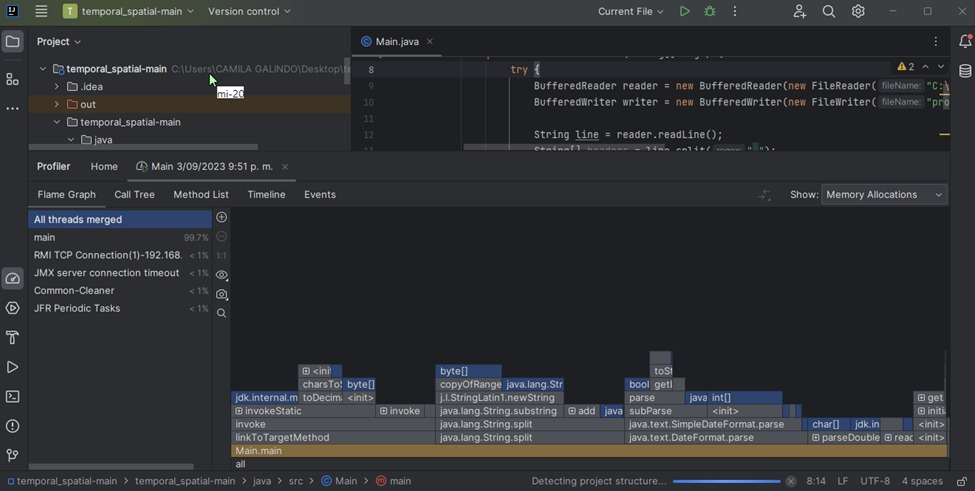
\includegraphics[width=0.9\linewidth]{Lenovo AMD 3020e/FlameGraph Memory Allocation 1.jpeg}
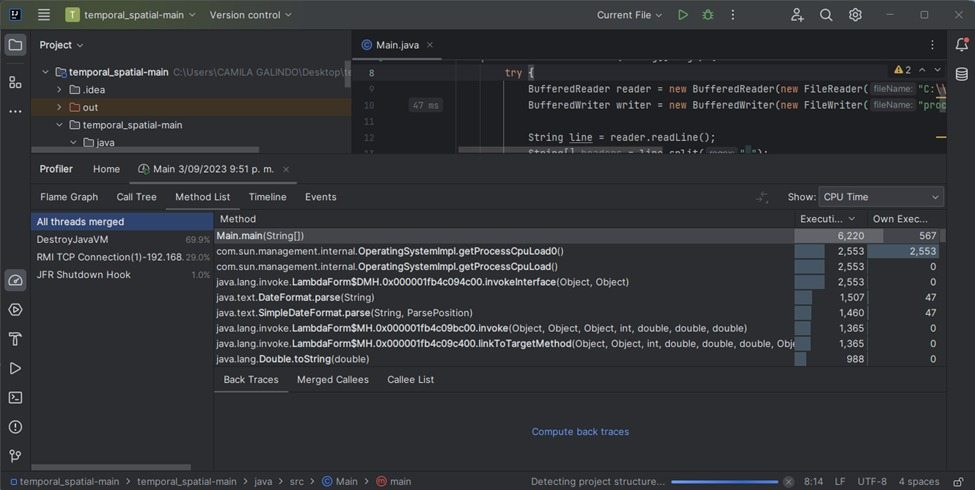
\includegraphics[width=0.9\linewidth]{Lenovo AMD 3020e/Method List CPU Time 1.jpeg}
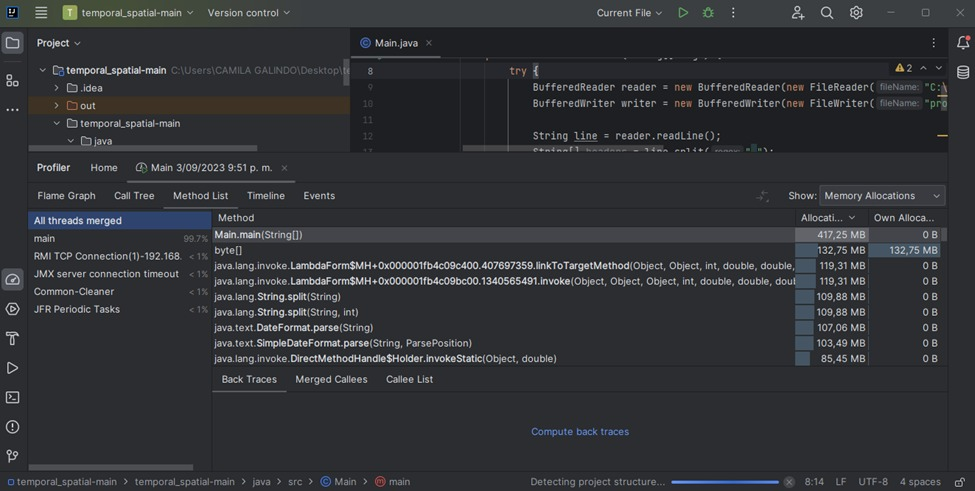
\includegraphics[width=0.9\linewidth]{Lenovo AMD 3020e/Method List Memory Allocation 1.jpeg}

\textbf{Ejecución 2\\}
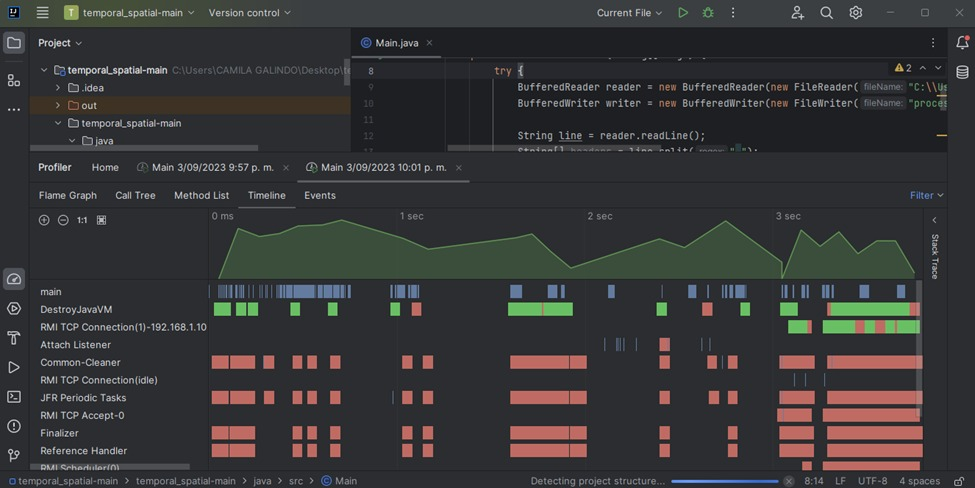
\includegraphics[width=0.9\linewidth]{Lenovo AMD 3020e/TimeLine 2.jpeg}
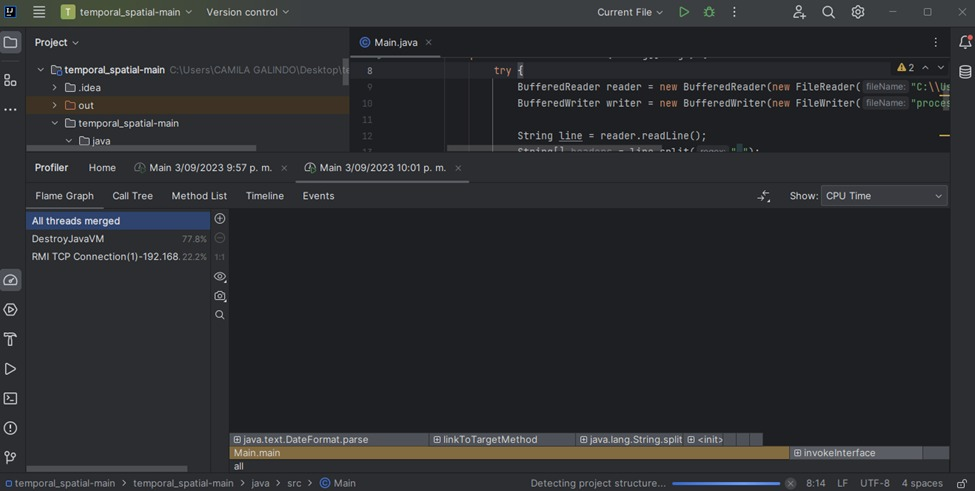
\includegraphics[width=0.9\linewidth]{Lenovo AMD 3020e/FlameGraph CPU Time 2.jpeg}
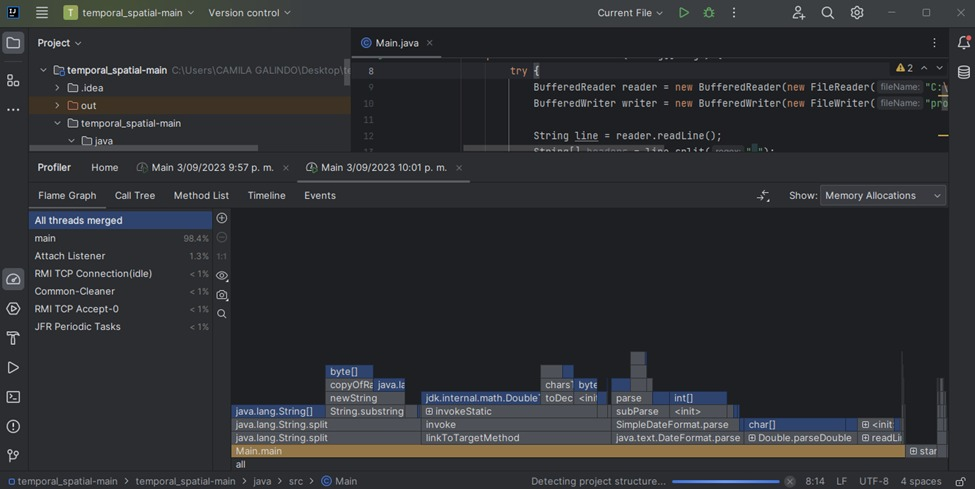
\includegraphics[width=0.9\linewidth]{Lenovo AMD 3020e/FlameGraph Memory Allocation 2.jpeg}
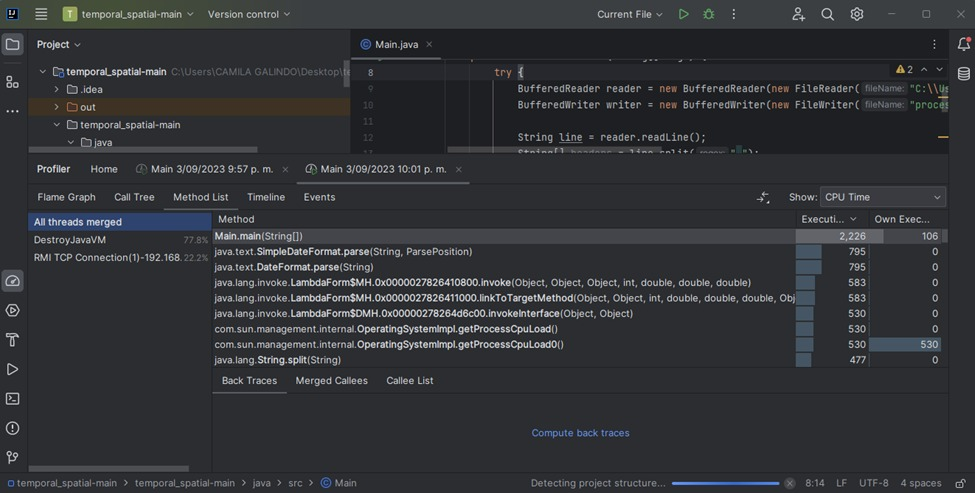
\includegraphics[width=0.9\linewidth]{Lenovo AMD 3020e/Method List CPU Time 2.jpeg}
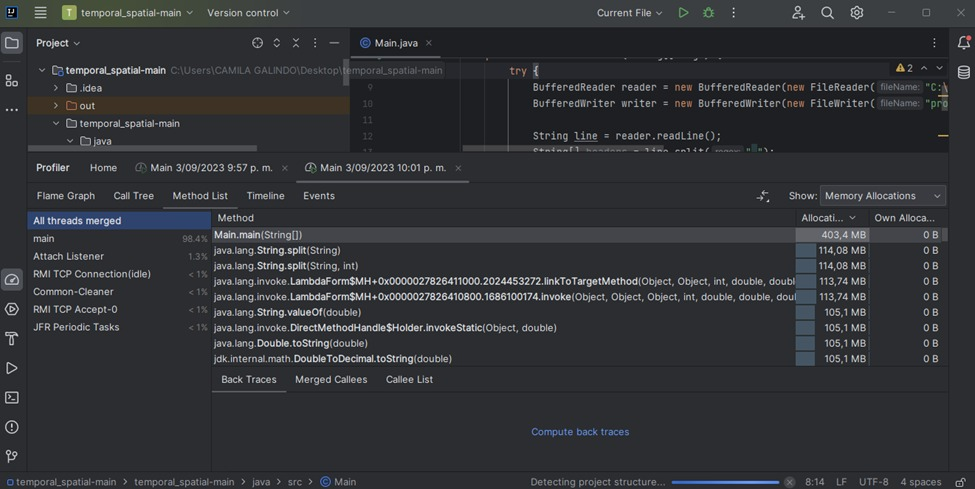
\includegraphics[width=0.9\linewidth]{Lenovo AMD 3020e/Method List Memory Allocation 2.jpeg}

\textbf{Ejecución 3\\}
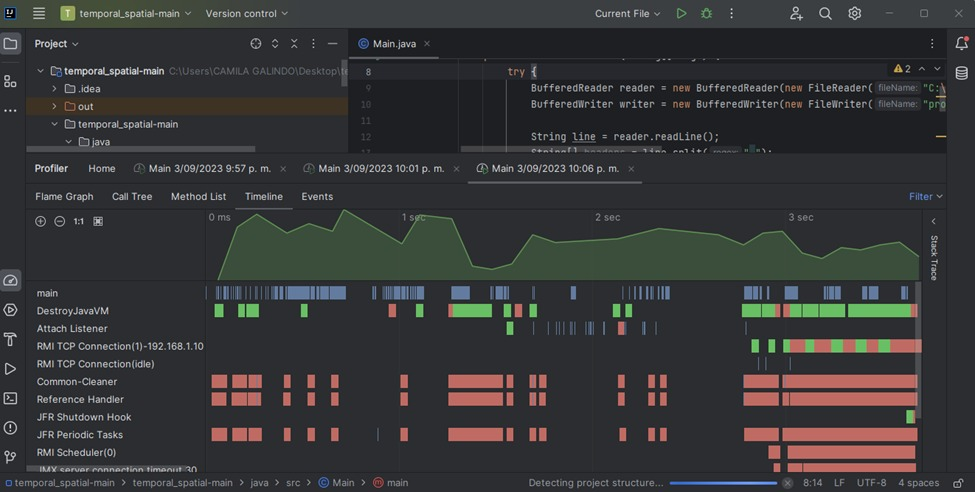
\includegraphics[width=0.9\linewidth]{Lenovo AMD 3020e/TimeLine 3.jpeg}
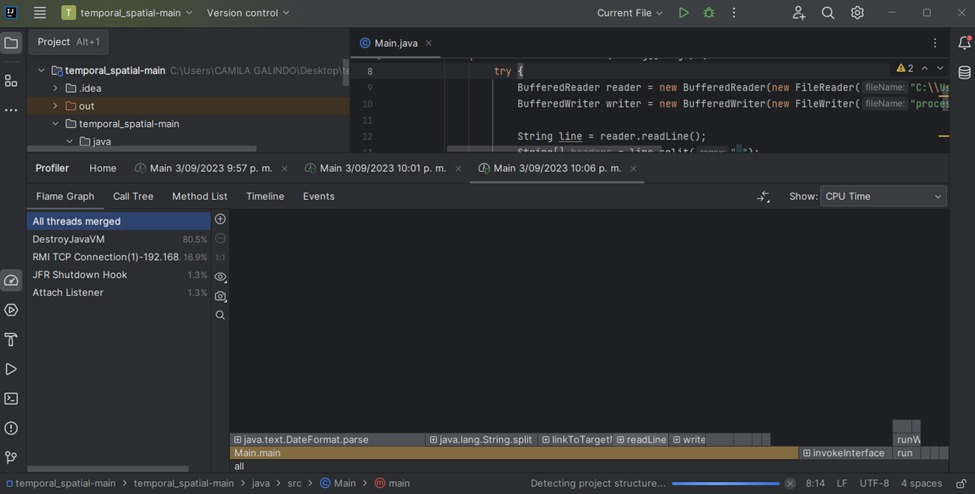
\includegraphics[width=0.9\linewidth]{Lenovo AMD 3020e/FlameGraph CPU Time 3.jpeg}
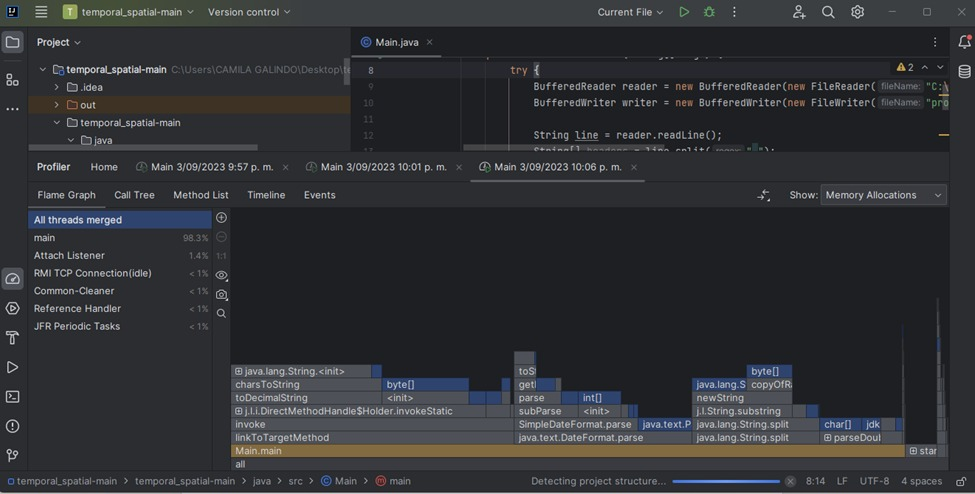
\includegraphics[width=0.9\linewidth]{Lenovo AMD 3020e/FlameGraph Memory Allocation 3.jpeg}
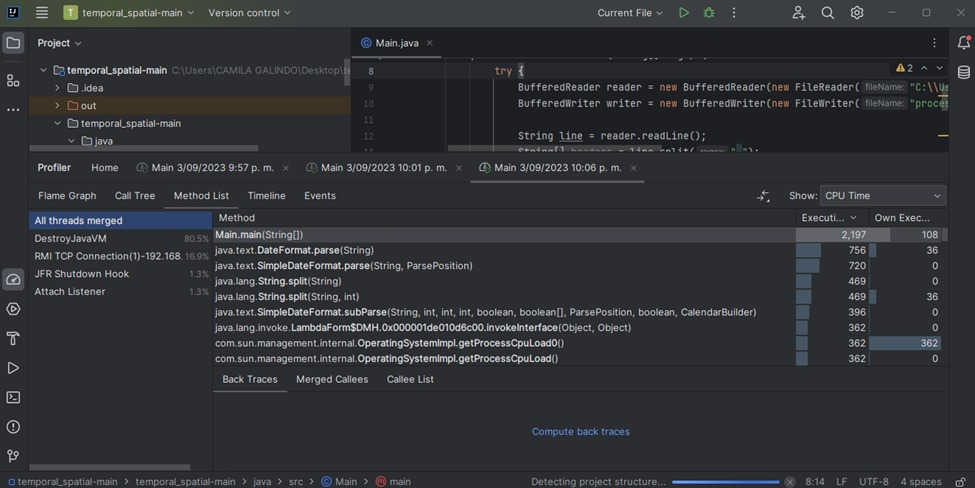
\includegraphics[width=0.9\linewidth]{Lenovo AMD 3020e/Method List CPU Time 3.jpeg}
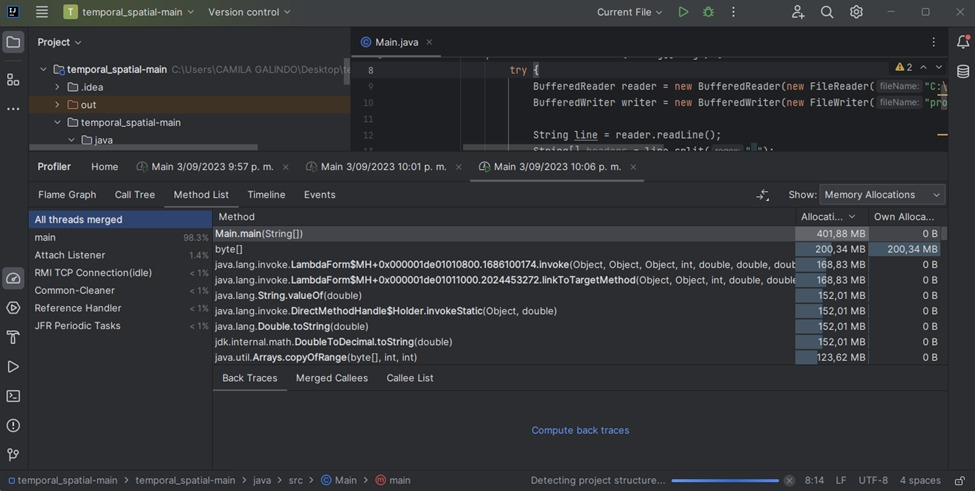
\includegraphics[width=0.9\linewidth]{Lenovo AMD 3020e/Method List Memory Allocation 3.jpeg}\\

\section{Resumen resultados espacio-temporales}

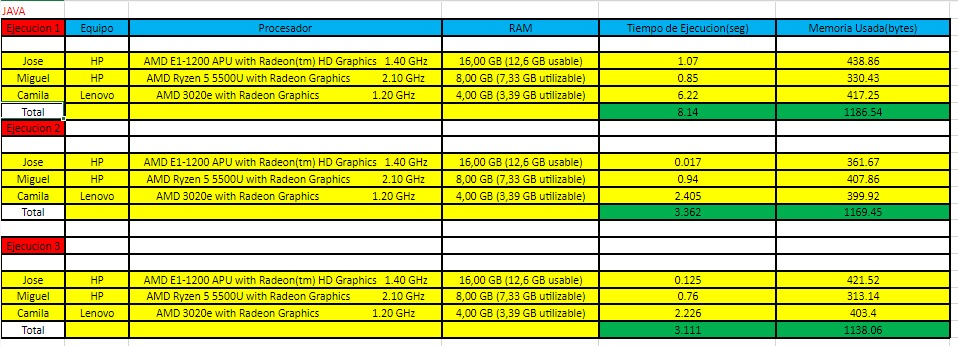
\includegraphics[width=1\linewidth]{Resultados finales.jpeg}

\section{Coclusiones}

En conclusión, la comprensión de estas dimensiones y su adecuada aplicación en la programación es esencial para el éxito de un proyecto de desarrollo de software en un mundo cada vez más dependiente de la tecnología, así como para la eficacia de las propias aplicaciones y que podamos ver que tan eficiente es un codigo comparado con otro, así mismo como sus diferencias entre equipos y las capacidades y requerimientos que cada programa exige a un dispositivo o equipo.

\section{Bibliografia}

\item https://github.com

\end{document}


